\documentclass[a4paper, 14pt]{extarticle}
\usepackage[utf8]{inputenc}
\usepackage[paper=a4paper, top=1cm, right=1cm, bottom=1.5cm, left=2cm]{geometry}
\usepackage{setspace}
\onehalfspacing

\usepackage{graphicx}
\graphicspath{{plots/}, {images/}}

\parindent=1.25cm

\usepackage{titlesec}

\renewcommand{\thesection}{\arabic{section}.}
\renewcommand{\thesubsection}{\arabic{section}.\arabic{subsection}.}

\titleformat{\section}
    {\normalsize\bfseries}
    {\thesection}
    {1em}{}

\titleformat{\subsection}
    {\normalsize\bfseries}
    {\thesubsection}
    {1em}{}

% Настройка вертикальных и горизонтальных отступов
\titlespacing*{\subsection}{\parindent}{*4}{*4}

\usepackage[square, numbers, sort&compress]{natbib}
\makeatletter
\bibliographystyle{unsrt}
\renewcommand{\@biblabel}[1]{#1.} 
\makeatother

\newcommand{\maketitlepage}[6]{
    \begin{titlepage}
        \singlespacing
        \newpage
        \begin{center}
            Министерство образования и науки Российской Федерации \\
            Федеральное государственное бюджетное образовательное \\
            учреждение высшего профессионального образования \\
            <<Волгоградский государственный технический университет>> \\
            #1 \\
            Кафедра #2
        \end{center}


        \vspace{14em}

        \begin{center}
            \large Семестровая работа по дисциплине: #6
            \\ Тема <<#3>>
        \end{center}

        \vspace{5em}

        \begin{flushright}
            \begin{minipage}{.5\textwidth}
                Выполнил: \\#4\\
                Дата сдачи:\\
                \\
                Проверила: #5\\
                Дата отчета:\\
                \\
                Отчет приняла:\\
                Оценка \underline{\ \ \ \ \ \ \ \ \ \ \ \ \ \ \ \ \ \ \ \ \ \ \ 
                \ \ \ \ \ \ \ \ \ }
            \end{minipage}
        \end{flushright}

        \vspace{\fill}

        \begin{center}
            Волгоград, \the\year
        \end{center}

    \end{titlepage}
    \setcounter{page}{2}
}

\newcommand{\maketitlepagefemale}[6]{
    \begin{titlepage}
        \singlespacing
        \newpage
        \begin{center}
            Министерство образования и науки Российской Федерации \\
            Федеральное государственное бюджетное образовательное \\
            учреждение высшего профессионального образования \\
            <<Волгоградский государственный технический университет>> \\
            #1 \\
            Кафедра #2
        \end{center}


        \vspace{14em}

        \begin{center}
            \large Семестровая работа по дисциплине: #6
            \\ Тема <<#3>>
        \end{center}

        \vspace{5em}

        \begin{flushright}
            \begin{minipage}{.4\textwidth}
                Выполнила:\\#4\\
                Дата сдачи:\\
                \\
                Проверила: #5\\
                Дата отчета:\\
                \\
                Отчет приняла:\\
                Оценка \underline{\ \ \ \ \ \ \ \ \ \ \ \ \ \ \ \ \ \ \ \ \ \ \ 
                \ \ \ \ \ \ \ \ \ }
            \end{minipage}
        \end{flushright}

        \vspace{\fill}

        \begin{center}
            Волгоград, \the\year
        \end{center}

    \end{titlepage}
    \setcounter{page}{2}
}

\input{../../.preambles/10-russian}
\input{../../.preambles/20-math}

\usepackage{color}
\definecolor{darkgreen}{rgb}{0,.5,0}
\usepackage[colorlinks,linkcolor=black,filecolor=blue,citecolor=darkgreen]{hyperref}

\renewcommand{\labelitemi}{\normalfont\bfseries{--}}
\newcommand{\st}[1]{\bar{#1}}
\newcommand{\ds}{\displaystyle}

\begin{document}
\maketitlepage{Факультет электроники и вычислительной техники}{физики}
{Мультистационарные системы. Отбор одного\\из равноправных. Биологическая
дифференциация}{студент~группы~Ф-369~Чечеткин~И.~А.}{доцент Грецова~Н.~В.}
{биофизика}
        
    \tableofcontents
    \thispagestyle{empty}
    \newpage
    \section{Цель работы}

Изучение методов определения статических характеристик триода и изучение
режимов его работы.

\section{Содержание работы}

\subsection{Основные сведения}

Триод является вакуумным электронным прибором, отличающимся от диода наличием
третьего электрода, расположенного между катодом и анодом и называемого
управляющей сеткой или просто сеткой.

На рисунке~\ref{pic1} показаны распространенные конструкции электродов триода.
\begin{figure}[ht]
  \center
  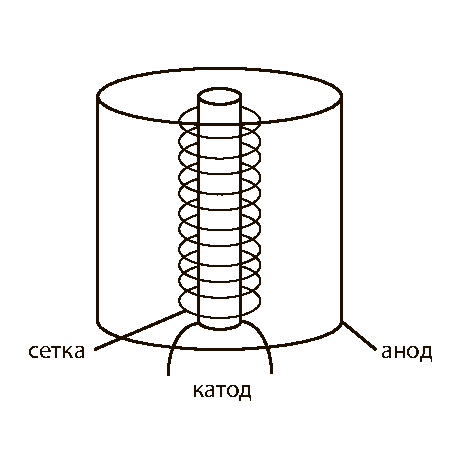
\includegraphics[width=.4\textwidth]{1_1} \hspace{2em}
  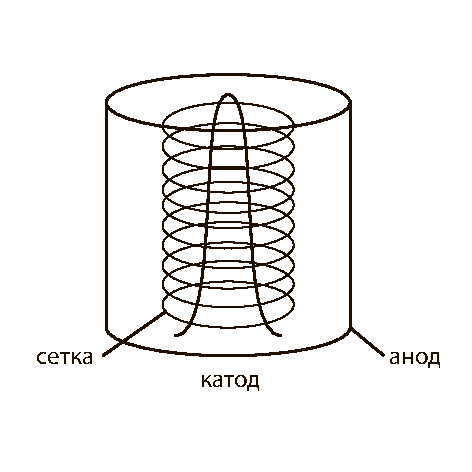
\includegraphics[width=.4\textwidth]{1_2}
  \caption{Конструкция электродов триода}
  \label{pic1}
\end{figure}

Действие управляющей сетки заключается в том, что она регулирует распределение
пространственного заряда между катодом и анодом и, таким образом, управляет
потоком электронов внутри лампы, то есть анодным током. Вследствие того, что
сетка не является сплошной, она свободно пропускает электроны, летящие к аноду.
С другой стороны, она формирует структуру поля, причем резко ослабляется
влияние изменения анодного напряжения на поле вблизи катода --- экранирует
катод от анода и ослабляет действие анода на электроны, вылетающие с катода.

Напряжением на сетке или сеточным напряжением называют разность потенциалов
между сеткой и катодом, то есть потенциал сетки относительно катода. В лампах
с катодом прямого накала все напряжения отсчитывают относительного
отрицательного конца катода.

На рисунке \ref{pic2} показано распределение поля в триоде при различных
величинах напряжения на сетке и фиксированном анодном напряжении. Видно, что
сетка задерживает большую часть поля. Чем гуще сетка, тем сильнее экранирует
она катод от влияния анода. Вследствие этого и отчасти потому, что сетка
расположена ближе к катоду, чем к аноду, небольшие изменения потенциала на
сетке оказывают гораздо более сильное действие на анодный ток, чем значительные
изменения потенциала на аноде.

\begin{figure}[ht]
  \center
  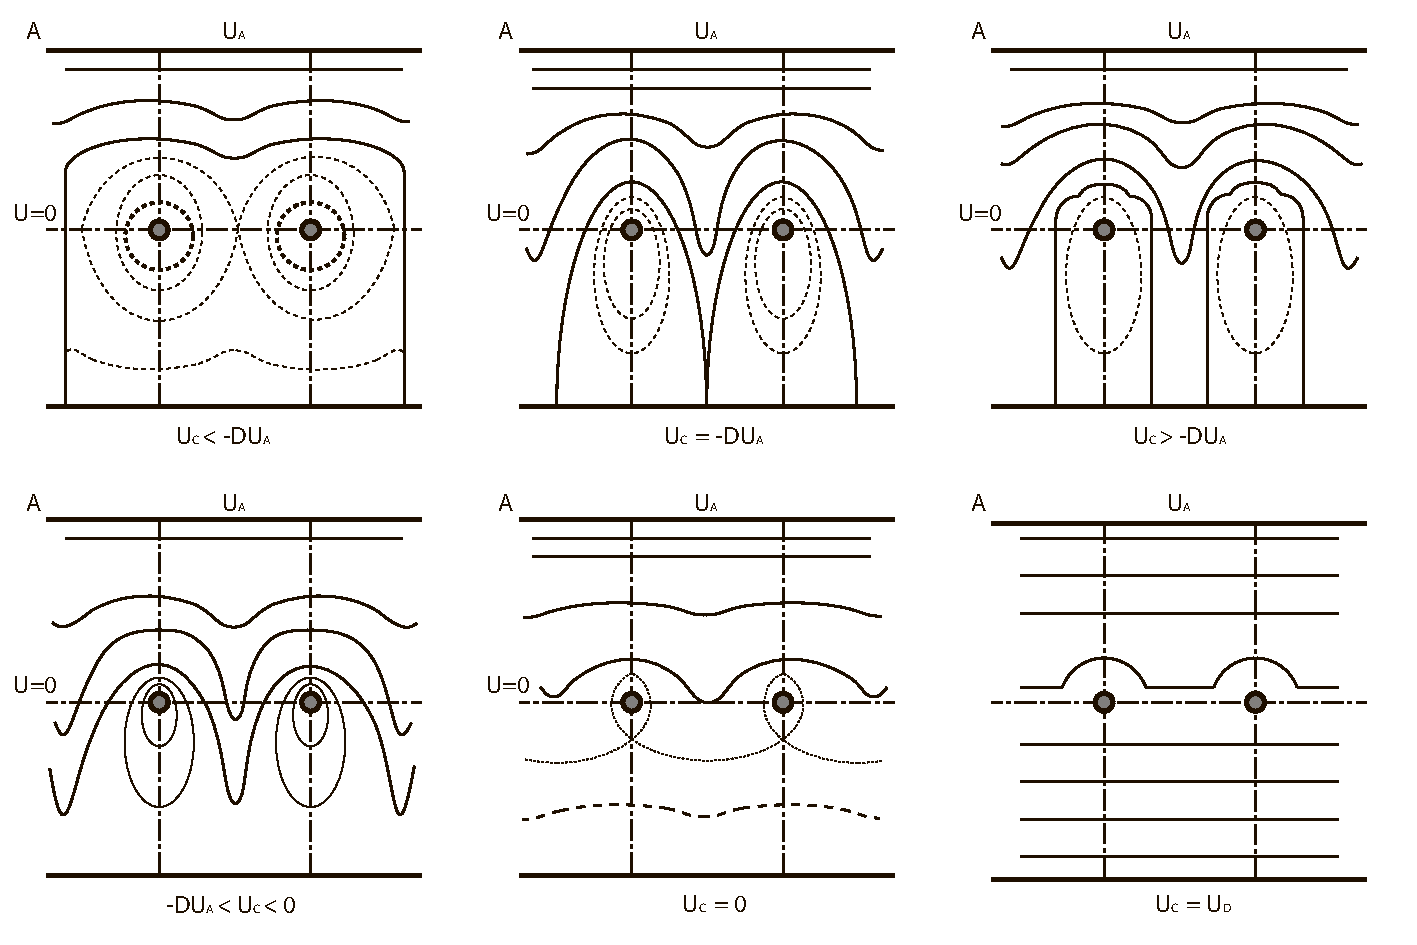
\includegraphics[width=.9\textwidth]{2}
  \caption{Распределение электростатического потенциала плоского триода при
  различных потенциалах сетки и одинаковом анодном напряжении}
  \label{pic2}
\end{figure}

При небольшом отрицательном напряжении сетка отталкивает электроны, но часть их
все же пролетает в ее просветы благодаря притяжению анода. Однако можно
увеличить отрицательное напряжение настолько, что она будет отталкивать все
электроны и анодный ток прекратится. Лампа будет заперта.

Прохождение анодного тока через триод можно описать, введя представление
эквивалентного диода, то есть такого диода, у которого плоскость анода
совпадает с плоскостью сетки в триоде. В этом случае катодный ток подчиняется
классическому закону Ленгмюра:
\begin{equation}
  I_k = P(U_C + DU_A)^{3/2}.
  \label{eq1}
\end{equation}

Здесь \( D \) -- проницаемость сетки, пропорциональная отношению диаметра сетки
к периоду ее намотки, \( P \) -- первеанс триода, зависящий от геометрических
размеров триода, \( U_C \) -- напряжение на сетке, \( U_A \) -- напряжение на
аноде.

В этом случае условие прекращение анодного тока соответствует равенству
\begin{equation}
  U_C = -DU_A.
  \label{eq2}
\end{equation}

При увеличении напряжения на сетке (но при условии, что \( U_C < 0 \)) анодный
ток совпадает по величине с катодным и растет по закону Ленгмюра \eqref{eq1}.

В результате характер изменения анодного тока в триоде может быть описан двумя
характеристиками: анодно-сеточной, когда при фиксированном анодном напряжении
изменяется напряжение на сетке (рисунок \ref{pic3}), и анодной, когда
напряжение на сетке остается постоянным, но варьируется величина напряжения на
аноде (рисунок \ref{pic4}). Обе характеристики взаимосвязаны~--- и по семейству
анодно-сеточных характеристик легко построить анодную.

\begin{figure}[ht]
  \center
  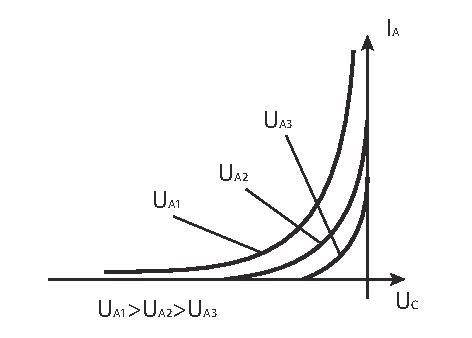
\includegraphics[width=.45\textwidth]{3} \hspace{2em}
  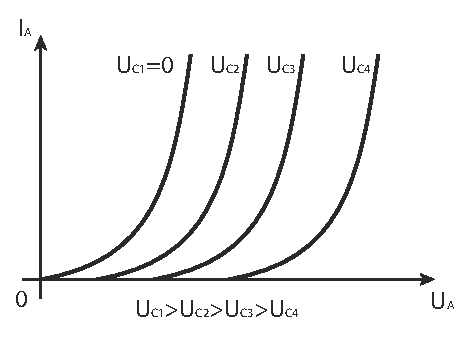
\includegraphics[width=.45\textwidth]{4}
  \parbox{.45\textwidth}{\caption{Семейство анодно-сеточных характеристик
  триода}\label{pic3}} \hspace{2em}
  \parbox{.45\textwidth}{\caption{Семейство анодных характеристик триода}
  \label{pic4}}
\end{figure}

Однако при положительных напряжениях на сетке картина существенно изменяется.
Когда \( U_A > U_D \), все электроны, пролетевшие плоскость сетки, попадают на
анод и сеточный ток определяется лишь теми электронами, которые перехватываются
сеткой при их прямом движении к аноду. Такой режим носит название \emph{режима
токоперехвата}. Он существует до тех пор, пока напряжение на аноде не
сравняется с действующим напряжением. Это означает, что граничный потенциал на
сетке определяется условием \( U_A = U_D \), или
\[
  \left( \frac{U_A}{U_C} \right)_\emph{гр} = \frac{\sigma}{1 - D\sigma}.
\]

Здесь \( \sigma \) -- параметр, который носит название остроты управления и
равный приблизительно величине \( \sigma = 1/(1 + D) \). А начинается этот
режим при положительных напряжениях на сетке.

Введем коэффициент токопрохождения \( s = I_a/I_k \) и коэффициент
токораспределения \( k = I_a/I_c \). Оба эти коэффициента равнозначны, но чаще
используют коэффициент \( s \), зная который легко определяются величины всех
токов:
\[
  I_a = s I_k; \qquad I_c = (1 - s) I_k.
\]

Самая простая оценка величины коэффициента токопрохождения в режиме
токоперехвата может быть сделана при сравнении характера траекторий электронов,
когда напряжение на сетке равно действующему: \( U_C = U_D \), или
\[
  \left( \frac{U_A}{U_C} \right)_1 = \left( \frac{1}{\sigma} - 1 \right)
  \frac{1}{D}; \qquad s = s_1.
\]

В этом случае распределение потенциала в плоском триоде практически совпадает
с распределением потенциала в плоском диоде с расстоянием между анодом и катодом
равном расстоянию между сеткой и катодом. При
\( \left( \cfrac{U_C}{U_D} \right) < 1 \) витки сетки отталкивают электроны,
число электронов, перехватываемых сеткой, уменьшается и \( s \) становится
больше \( s_1 \). При \( \left( \cfrac{U_C}{U_D} \right) > 1 \) витки сетки
начинают играть роль рассеивающей линзы.

Оценить величину коэффициента токопрохождения можно достаточно просто. В случае
\( s = s_1 \) на сетку будут попадать лишь те электроны, которые вылетают из
катода прямо под сеткой. Тогда, если эмиссия из катода равномерна,
\( s_1 = 1 - \cfrac{2R_C}{L} \). При \( \left( \cfrac{U_C}{U_D} \right) < 1 \)
коэффициент токопрохождения растет, при
\( \left( \cfrac{U_C}{U_D} \right) > 1 \) -- падает, причем изменение \( s \)
связано с изменением эффективного электрического радиуса сетки
\( R_{C\,\text{эфф}} \) -- радиуса, который определяет попадание электрона на
сетку.

Когда \( U_D > U_A \), в промежутке между сеткой и анодом на электроны
действует тормозящее поле и не все электроны долетают до анода. Такой режим
носит название \emph{режима возврата электронов}. Ток сетки при этом в основном
определяется теми электронами, которые возвращаются от анода к сетке.

На рисунке \ref{pic5} приведены типичные кривые токораспределения (без учета
начальных скоростей электронов и полей пространственного заряда).

\begin{figure}[ht]
  \center
  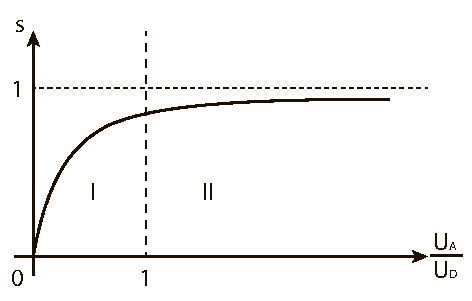
\includegraphics[width=.5\textwidth]{5}
  \caption{Кривая токораспределения в плоском триоде\\
  1 -- область возврата электронов; 2 -- область токоперехвата}
  \label{pic5}
\end{figure}

\section{Описание экспериментальной установки}

На рисунке~\ref{picLook} приведен внешний вид экспериментальной установки по
изучению статических характеристик триода.

\begin{figure}[ht]
  \center
  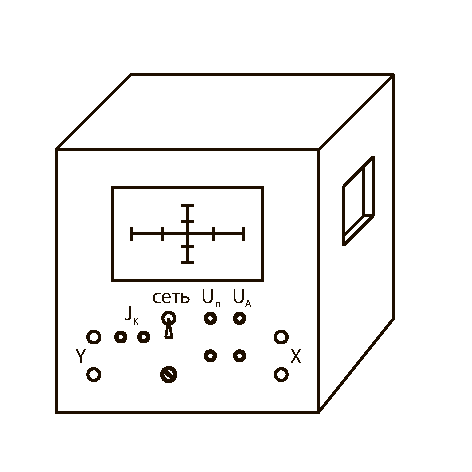
\includegraphics[width=.39\textwidth]{look} \hfill
  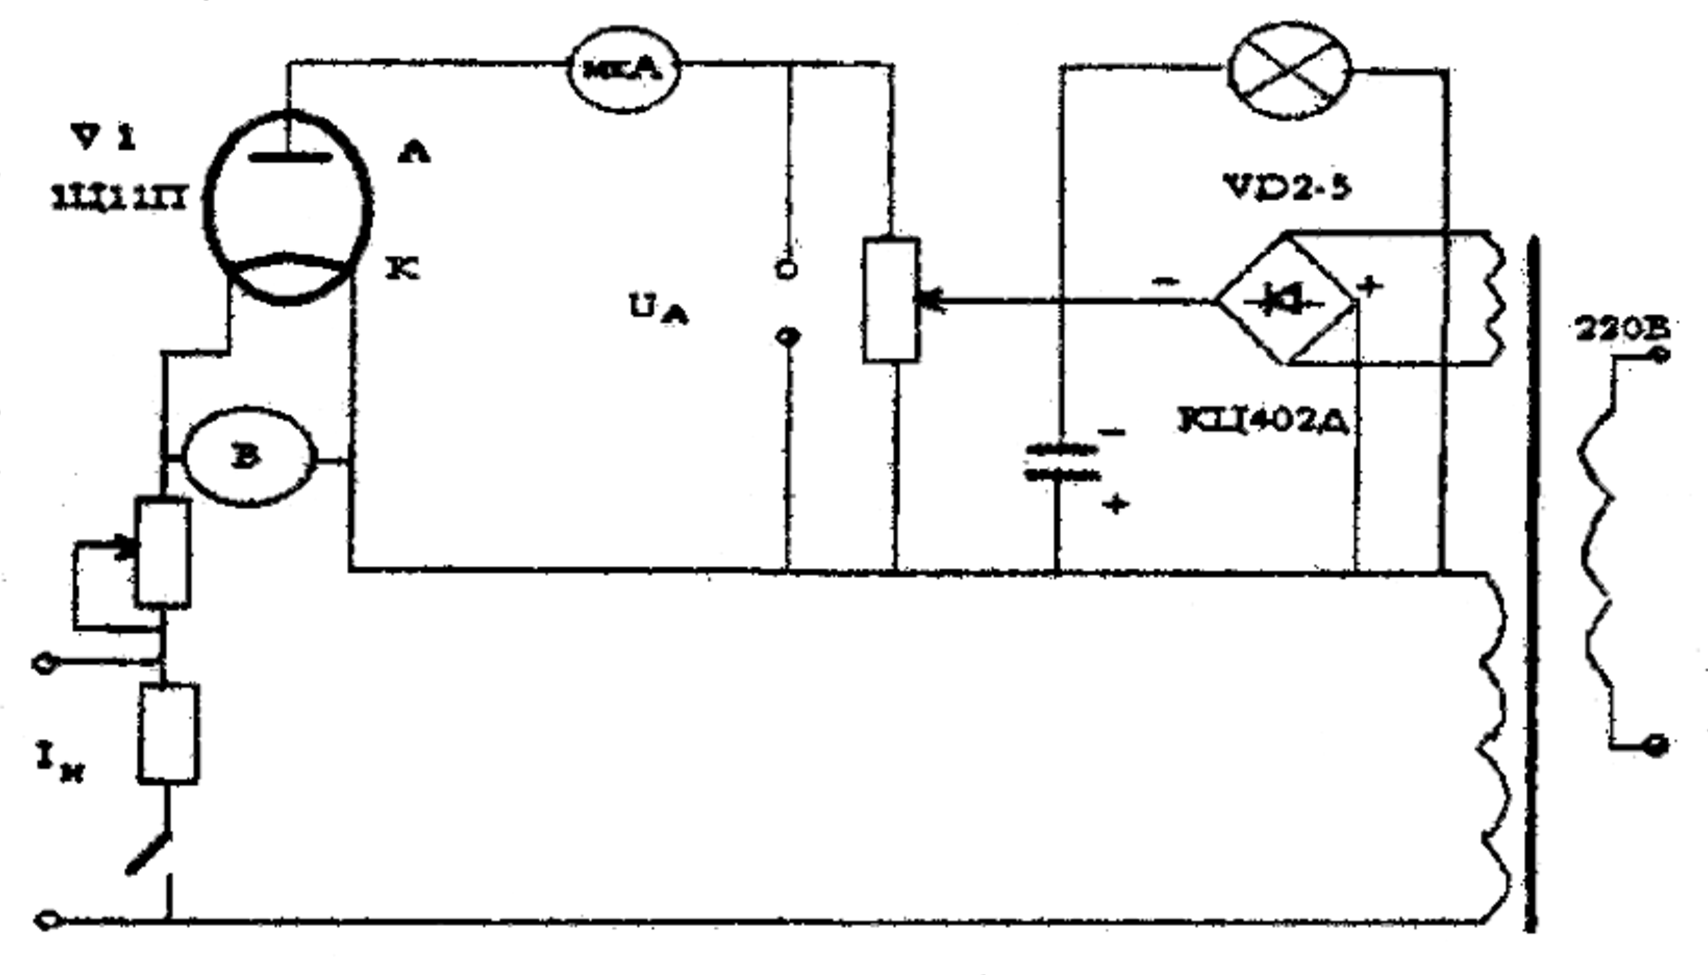
\includegraphics[width=.6\textwidth]{scheme} \\
  \parbox{.39\textwidth}{\caption{Внешний вид экспериментальной установки}
      \label{picLook}} \hfill
  \parbox{.6\textwidth}{\caption{Принципиальная электрическая схема
      установки} \label{picScheme}}
\end{figure}

\begin{enumerate}
  \item Вакуумный триод.
  \item Вольтметр.
  \item Амперметр.
  \item Регулятор сеточного напряжения.
  \item Регулятор анодного напряжения.
  \item Переключатель измеряемого напряжения.
  \item Выключатель сетевого напряжения.
\end{enumerate}

Принципиальная схема экспериментальной установки представлена на
рисунке~\ref{picScheme}.

\section{Методика проведения эксперимента}
\renewcommand{\labelenumi}{4.\arabic{enumi}.}
\begin{enumerate}
  \item Включив сеть, дать прибору прогреться не менее 3~мин.
  \item Переключатель~6 должен находиться в положении <<\( U_A \)>>, а
    регулятор~4 должен быть повернут влево до упора.
  \item Подать на анод максимально возможное напряжение регулятором~5
    (\( U_{a_m} \sim \)40~В). Зафиксировать значение анодного тока.
  \item Переключив тумблер~6 в положение <<\( U_C \)>>, повысить по модулю
    напряжение на сетке на одно деление регулятором~4. Переключить~6 в положение
    <<\( U_A \)>> и регулятором~5 вернуть напряжение на аноде к \( U_{a_m} \).
    Записать значение анодного тока.
  \item Повторяя пункт~4 для различных \( U_{a_m} \), снять зависимость
    \( I_a(U_c) \) при \( U_a = \const \). Данные занести в
    таблицу~\ref{web-anod}.

    \begin{table}[ht]
      \center
      \caption{Семейство анодно-сеточных характеристик}
      \label{web-anod}
      \begin{tabular}{|m{.1\textwidth}|C{.1}|*{7}{C{.07}|}} \hline
        \multirow{5}{*}{\( U_{a_{01}} \)} &
          \( U_c \),~В &&&&&&& \\ \cline{2-9}
        & \( I_{a_1} \),~мА &&&&&&& \\ \cline{2-9}
        & \( I_{a_2} \),~мА &&&&&&& \\ \cline{2-9}
        & \( I_{a_3} \),~мА &&&&&&& \\ \cline{2-9}
        & \( \average{I_a} \),~мА &&&&&&& \\ \hline
        \multirow{4}{*}{\( U_{a_{02}} \)} &
          \( U_c \),~В &&&&&&& \\ \cline{2-9}
        \multirow{4}{*}{и т.~д.} &
          \( I_{a_1} \),~мА &&&&&&& \\ \cline{2-9}
        & \( I_{a_2} \),~мА &&&&&&& \\ \cline{2-9}
        & \( I_{a_3} \),~мА &&&&&&& \\ \cline{2-9}
        & \( \average{I_a} \),~мА &&&&&&& \\ \hline
      \end{tabular}
    \end{table}

  \item Зафиксировав напряжение на сетке регулятором~4, изменять напряжение на
    аноде регулятором~5 и снять зависимость \( I_a(U_a) \) при
    \( U_c = \const \).
  \item Повторить пункт~6 для различных напряжениях на сетке \( U_c = \const \).
    Результаты занести в таблицу~\ref{anod-anod}.
    
    \begin{table}[ht]
      \center
      \caption{Семейство анодных характеристик триода}
      \label{anod-anod}
      \begin{tabular}{|m{.1\textwidth}|C{.1}|*{7}{C{.07}|}} \hline
        \multirow{5}{*}{\( U_{c_{01}} \)} &
          \( U_a \),~В &&&&&&& \\ \cline{2-9}
        & \( I_{a_1} \),~мА &&&&&&& \\ \cline{2-9}
        & \( I_{a_2} \),~мА &&&&&&& \\ \cline{2-9}
        & \( I_{a_3} \),~мА &&&&&&& \\ \cline{2-9}
        & \( \average{I_a} \),~мА &&&&&&& \\ \hline
        \multirow{4}{*}{\( U_{c_{02}} \)} &
          \( U_a \),~В &&&&&&& \\ \cline{2-9}
        \multirow{4}{*}{и т.~д.} &
          \( I_{a_1} \),~мА &&&&&&& \\ \cline{2-9}
        & \( I_{a_2} \),~мА &&&&&&& \\ \cline{2-9}
        & \( I_{a_3} \),~мА &&&&&&& \\ \cline{2-9}
        & \( \average{I_a} \),~мА &&&&&&& \\ \hline
      \end{tabular}
    \end{table}
    
    \item Построить графики анодно-сеточной и анодной характеристик на
      миллиметровой бумаге.
    \item По экспериментально определенным анодно-сеточным характеристикам
      построить семейство анодных характеристик и сравнить с анодными
      характеристиками, полученными экспериментально.
\end{enumerate}

\section*{Вопросы для самопроверки}
\vspace{-1.5em}
\renewcommand{\labelenumi}{\arabic{enumi}.}
\begin{enumerate}
  \singlespacing
  \itemsep -.5pt
  \item Какова роль сетки в триоде?
  \item Что такое эквивалентный диод?
  \item Опишите распределение потенциала в триоде для различных соотношений
    потенциалов на сетке и на аноде.
  \item Какие характеристики описывают работу триода?
  \item Как на базе анодно-сеточных характеристик построить семейство
    анодных характеристик?
  \item Основные схемы включения триода в радиотехническую цепь (схема
    усилителя с общим катодом, с общим анодом, с общей сеткой).
  \item Опишите особенности анодных характеристик генераторного триода.
\end{enumerate}

\section*{Список рекомендуемой литературы}
\vspace{-1.5em}
\begin{enumerate}
  \singlespacing
  \itemsep -.5pt
  \item Шеин~А.~Г. Вакуумная и газоразрядная электроника. Ч. 1.: учеб.
  пособие~/ А.~Г.~Шеин, Д.~Г.~Ковтун~--- Волгоград: ВолгГТУ. 2008.~--- 108с.
  \item Клейнер~Э.~Ю. Основы теории электронных ламп: учеб. пособие для
  вузов~/ Э.~Ю.~Клейнер~--- М.: Высш. шк. 1974.~--- 368с.
  \item Шимони~К. Физическая электроника~/ К.~Шимони, пер. с нем. под. ред.
  В.~Раховского~--- М.: Энергия. 1977.~--- 608c.
  \item Кацман~А.~М. Электронные лампы высоких и низких частот: учеб. пособие
  для вузов~/ А.~М.~Кацман~--- М.: Высш. шк. 1972.~--- 388с.
\end{enumerate}
\end{document}